%%%%%%%%%%%%%%%%%%%%%%%%%%%%%%%%%%%%%%%%%%%%%%%%%%%%%%%%%%%%%%%%%%%%%%%%%%%%%%%%
%2345678901234567890123456789012345678901234567890123456789012345678901234567890
%        1         2         3         4         5         6         7         8

\documentclass[letterpaper, 10 pt, conference]{ieeeconf}  % Comment this line out
                                                          % if you need a4paper
%\documentclass[a4paper, 10pt, conference]{ieeeconf}      % Use this line for a4
                                                          % paper

\IEEEoverridecommandlockouts                              % This command is only
                                                          % needed if you want to
                                                          % use the \thanks command
\overrideIEEEmargins
% See the \addtolength command later in the file to balance the column lengths
% on the last page of the document
\usepackage{amssymb,amsmath,graphicx,multicol,bm}
\usepackage[margin=.75in]{geometry}
%\usepackage[mathcal]{euscript}


% The following packages can be found on http:\\www.ctan.org
%\usepackage{graphics} % for pdf, bitmapped graphics files
%\usepackage{epsfig} % for postscript graphics files
%\usepackage{mathptmx} % assumes new font selection scheme installed
%\usepackage{times} % assumes new font selection scheme installed
%\usepackage{amsmath} % assumes amsmath package installed
%\usepackage{amssymb}  % assumes amsmath package installed

\title{\LARGE \bf
Approximate Latent State Transitions for Model-Based Reinforcement Learning
}

%\usepackage{amsthm}
\newtheorem{prop}{Proposition}

%\author{ \parbox{3 in}{\centering Huibert Kwakernaak*
%         \thanks{*Use the $\backslash$thanks command to put information here}\\
%         Faculty of Electrical Engineering, Mathematics and Computer Science\\
%         University of Twente\\
%         7500 AE Enschede, The Netherlands\\
%         {\tt\small h.kwakernaak@autsubmit.com}}
%         \hspace*{ 0.5 in}
%         \parbox{3 in}{ \centering Pradeep Misra**
%         \thanks{**The footnote marks may be inserted manually}\\
%        Department of Electrical Engineering \\
%         Wright State University\\
%         Dayton, OH 45435, USA\\
%         {\tt\small pmisra@cs.wright.edu}}
%}

\author{Ryan Theisen}%$^{1}$% <-this % stops a space
%\thanks{$^{1}$Arizona State University, ryan.theisen@asu.edu}}


\begin{document}



\maketitle
\thispagestyle{empty}
\pagestyle{empty}


%%%%%%%%%%%%%%%%%%%%%%%%%%%%%%%%%%%%%%%%%%%%%%%%%%%%%%%%%%%%%%%%%%%%%%%%%%%%%%%%
\begin{abstract}

We explore a technique to model state transitions for use in model-based reinforcement learning. We use a latent encoding of the state space to model a transition distribution between states conditioned on actions. We show that, in addition to being used in a fully model based setting, this method can be used to augment a variety of different reinforcement learning techniques.

\end{abstract}


%%%%%%%%%%%%%%%%%%%%%%%%%%%%%%%%%%%%%%%%%%%%%%%%%%%%%%%%%%%%%%%%%%%%%%%%%%%%%%%%
\section{INTRODUCTION}

In model based reinforcement learning (RL), the representative agent is assumed to have full knowledge of the state-transition distribution $p(s'|s,a)$. For example, in Q-learning, the agent can learn the optimal policy $\pi$ by iteratively applying the Bellman backup equation:
\begin{align*}
	Q(s,a) = R(s) + \gamma\mathbb{E}_{s'\sim p(s'|s,a)}[\text{argmax}_{a'}Q(s',a')]
\end{align*}
where $\pi(s) = \text{argmax}_{a}Q(s,a)$. However, in most real-world cases, the state transition dynamics are unknown, leading to alternate approaches to the RL problem, which are unable to make use of the information provided by $p(s'|s,a)$.

We propose a new method for estimating the state transition distribution, except defining the transition instead on a latent representation $z\in\mathcal{Z}$ of the actual state $s\in\mathcal{S}$. Approaches to encoding input in such a way have been widely studied in the machine learning literature, and have been shown to be useful estimators of the latent data manifold. For examples, in variational autoencoders (VAEs), the latent distribution $p(z|x)$ is derived by minimizing a variation lower bound of the data likelihood. We employ a similar approach to encode the state $s$ into a latent distribution $p(z|s)$, which is in turn used to estimate a distribution $p(z'|z,a)$ that approximates the transition dynamics $p(s'|s,a)$.

\section{BACKGROUND}
*to do*

\section{GENERATING APPROXIMATE LATENT STATE TRANSITIONS}

\subsection{General Method}
%Consider the problem of representing the state $s\in\mathcal{S}$ by a probability distribution over a latent encoding, $p(z|s)$. Two desirable properties for such a representation to have are \textit{sufficiency} and \textit{minimality}. One says that a representation $z$ is \textit{sufficient} for a task $y$ if $I(y;s) = I(y;z)$. A representation $z$ of the state $s$ is \textit{minimal} if $I(s;z)$ is a small as possible while satisfying sufficiency. In particular, in this work, we consider the task of estimating the transition probability from a latent state $z \in \mathcal{Z}$ into another state $z'\in\mathcal{Z}$ after conditioning on an action $a\in\mathcal{A}$. In this case, the sufficiency condition is reduced to minimizing the conditional entropy $H(s'|z')$ and $H(z'|z)$; that is, we would like $z'$ to encode as much information about the state as possible and similarly that $z$ encode as much information about the transition to $z'$ as possible.

%Furthermore, we would like that our representations $z$ and $z'$ are jointly minimal; that is, $I(s;z), I(z;z')$ are as small as possible given (1)-(2) hold. (Achille and Soatto 2017) showed that the Information Bottleneck (IB) Lagrangian (Tibshy et al)
%\begin{align*}
%\mathcal{L}(\theta) = \eta_1H(s'|z') + \eta_2 H(z'|z) + \beta_1I(s;z) + \beta_2I(z;z')
%\end{align*}
%yields representations that are both sufficient and minimal. 

Let $(s, a, s')$, be a sample trajectory where $s'\sim p(s'|s,a)$. We would like that $p(z'|z,a)$ models the transition dynamics $p(s'|s,a)$ as closely as possible. We model this with the following
\begin{align*}
	\mathcal{L}_T(\theta, \phi) = \frac{1}{N}\sum_{i=1}^N \|\mathbb{E}[f_\theta(s')] - z'_i\|_2
\end{align*}
where $z'_1,...,z'_N \sim p(z'|z,a)$. Here we consider $s'$ to be a point estimate of $\mathbb{E}[p(s'|s,a)]$, with $f_\theta(s') \sim p(z|s')$ the latent encoding of this estimate.

Furthermore, we would like that the latent encoding $p(z|s)$ encodes as little information about the state as possible while still being sufficient to recover the transition. One way to do this is to penalize mutual information between the encoding $z$ and the state $s$; that is, we want to make
\begin{align*}
	\mathcal{L}_f(\theta) &= I(z;s) = \mathbb{E}_{s\sim p(s)}[D_{KL}(p_\theta(z|s)\| p(z)]\\
	&\approx \frac{1}{M}\sum_{j=1}^M D_{KL}(p_\theta(z|s_i)\| p(z))
\end{align*} 
where $p(z)$ is a prior on the latent encoding $z$. Such a penalty is known to be an effective regularizer of the state-encoder $f_\theta$.
\begin{figure}[t]
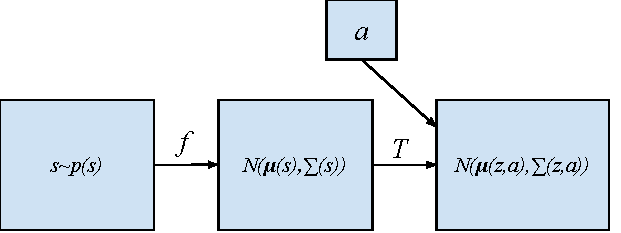
\includegraphics[width=8cm]{latentTransitionModelSimple.pdf}
\caption{A diagram of the latent transition model. In practice, $f_\theta$ and $T_\phi$ are parameterized as neural networks that output the mean and covariance of Gaussian distributions.}
\centering
\end{figure}

We then consider the aggregate objective
\begin{align*}
	\mathcal{L}(\theta,\phi) = \mathcal{L}_T(\theta,\phi) + \beta\mathcal{L}_f(\theta)
\end{align*}

%Because we are interested in modeling the transition $p(s'|s,a)$, we would like to be able to additionally condition $p(z'|z)$ on the action $a$. To do this, we condition on the action when estimating $p(z'|z)$, and then when evaluating the objective, marginalize out the action via the following decomposition:
%\begin{align*}
%p(z'|z) = \int_{\mathcal{A}}p(z'|z,a)p(a)da
%\end{align*}
%When $\mathcal{A}$ is finite, and actions are chosen at random, this reduces to 
%\begin{align*}
%p(z'|z) = \frac{1}{M} \sum_{j=1}^M p(z'|z,a_j)
%\end{align*}
%When $\mathcal{A}$ is not finite, or it is sufficiently large to render the above method computationally infeasible, a Monte Carlo approximation can be used.


\subsection{Special case: $\mathcal{A}$ finite and $p(z|s),\,p(z'|z,a)$ Gaussian}
As stated above, if the action space $\mathcal{A} = \{a_1,...,a_M\}$ is finite, and actions are taken at randomly, we have
\begin{align*}
	p(z'|z) = \frac{1}{M}\sum_{j=1}^M p(z'|z, a_j)
\end{align*}
In the case when $p(z'|z,a)$ is Gaussian, we have that $p(z'|z)$ is a finite sum of Gaussians and hence Gaussian itself. Furthermore, if the prior $p(z')$ is also Gaussian, then the KL divergence term can be computed analytically. The same is true whenever $p(z|s)$ and $p(z)$ are both Gaussians (see appendix).

\subsection{Trajectory Estimation and Planning}
One useful property of our design if that, if $p(z)$ and $p(z')$ are chosen to correspond, and $p(z'|z)$ and $p(z|s)$ are minimal, then one can consider estimating multiple steps into the future by applying $p(z'|z,a)$ iteratively. That is, given $z \sim p(z)$, one has that $z' \sim p(z'|z)$ can be used to sample $z''\sim p(z''|z',a)$ given some action $a$.

**It would be nice to have some theory justifying this, rather than just intuition**

\section{EXAMPLE: MODEL-BASED Q-LEARNING}
\subsection{Estimating Reward Function}

Given trajectories $(s,a,s',r)$ and a state encoder $f:\mathcal{S}\rightarrow\mathcal{Z}$, we can estimate a reward function $R: \mathcal{S}\rightarrow \mathbb{R}$ with $R(s) = R_\theta \circ f(s)$ where $R_\theta:\mathcal{Z}\rightarrow \mathbb{R}$ is taken to be a neural network with parameters $\theta$ (see Deep Mind paper). $R_\theta(z)$ can then be used to evaluate rewards of latent state transitions. $R_\theta$ can be trained straightforwardly using supervised learning.

\subsection{Monte Carlo Model-Based Q Learning}

Consider the standard Bellman Equation:
\begin{align*}
	Q(s,a) = R(s) + \gamma\mathbb{E}_{s'\sim p(s'|s,a)}[\text{argmax}_{a'}Q(s',a')]
\end{align*}
Under the hypothesis that the representation $z$ is sufficient for the given task, we can reframe this problem in terms of the latent encoding $z$:
\begin{align*}
	Q(z,a) &= R(z) + \gamma\mathbb{E}_{z'\sim p(z'|z,a)}[\text{argmax}_{a'}Q(z',a')]\\
	&= R(z) + \gamma\int_\mathcal{Z} \text{argmax}_{a'}Q(z',a')p(z'|z,a)dz'
\end{align*}
Since $p(z'|z,a)$ is known, we can estimate this integral using a Monte Carlo approach:
\begin{align*}
	Q(z,a) &= R(z) + \gamma\int_\mathcal{Z} \text{argmax}_{a'}Q(z',a')p(z'|z,a)dz'\\
	&\approx R(z) + \frac{\gamma}{N}\sum_{k=1}^N \text{argmax}_{a'}Q(z_k',a')
\end{align*}
where $z'_1,...,z'_N \sim p(z'|z,a)$ and $R(z) \equiv R_\theta(z)$ is approximated by the method outlined in B.

Using this set up, we can estimate $Q$ using a modified version of the DQN algorithm, minimizing the objective
\begin{align*}
	\mathcal{L} = \frac{1}{2}\Big(Q(z,a)-\big(R(z) + \frac{\gamma}{N}\sum_{k=1}^N \text{argmax}_{a'}Q(z_k',a')\big)\Big)^2 
\end{align*}
Note that, unlike the standard DQN algorithm, given the distribution $p(z'|z,a)$ and the function $R(z)$, this formulation can be trained entirely off-line, with no active interaction with the environment.

\section{EXPERIMENTS}

\section{CONCLUSION AND FUTURE WORK}










\end{document}
